\chapter{实现}
\label{cha:impl}

\section{调度模拟}
    调度模拟部分主要处理四部分工作:
    \begin{enumerate}
        \setlength{\itemindent}{1em}
        \item {\bfseries 生成}:将用户输入的TensorFlow代码转化为数据流图的形式。
        \item {\bfseries 剪枝}:根据输入输出列表对数据流图进行剪枝,得到最小依赖集。
        \item {\bfseries 模拟}:动态模拟模型运行状况。
        \item {\bfseries 预测}:根据设定好的配置代入性能模型数据,预测性能。
    \end{enumerate}
    
    下面分别就四部分工作的实现进行讲解。

\subsection{生成}
    数据流图的生成,我们通过直接调用TensorFlow接口的方式进行。具体地,用户在按照正常使用TensorFlow的方式定义所需要的运算,创建会话(session),这时模拟器通过所创建的会话,拿到会话生成的默认图(default graph),再转化为图定义(graphdef)的形式,以JSON格式保存,作为下一步的输入。
    
    其中,通过直接转化得到的数据主要包括图的结构信息。例如图的所有节点列表,边列表,连接方式等。在我们的模型中,图以节点列表的形式进行组织。每个节点保存以下几项信息:节点名称,节点操作种类,节点入边集,节点出边集。
    
    由于直接通过TensorFlow中用户对计算过程的定义创建的图是不具有输入规模数据的,在使用模型的时候,用户还需要手动规定输入数据规模,作为后续操作提供参数。其中,输入规模参数与操作定义绑定。要求用户在定义计算操作的时候指定运算操作名称(name),在输入规模参数的同时通过运算操作名称定位数据流图中的节点,从而得到完整的数据流图及其参数。
    
\subsection{剪枝}
    剪枝操作在TensorFlow中是以深度优先搜索(DFS)进行的,在我的实验中,为了配合我的图存储方式,我使用广度优先搜索(BFS)进行实现。从计算输出点开始,反向进行广度优先搜索。没有被覆盖到的节点直接删除。
    
    实际使用的情况下,正常定义的卷积神经网络是不需要这一步操作的,因为正常定义的网络并没有冗余节点。

\subsection{模拟}
    在得到剪枝后的模型后,我们需要根据TensorFlow实际的运行方式进行模拟,以求在静态环境下尽量还原TensorFlow的动态调度过程。
    
    模拟过程中,我们首先会创建若干资源标记,包括CPU线程和GPU。以我们的测试环境为例,我们的测试环境包含32个CPU线程和4个GPU。由于TensorFlow的会话在进行的时候,会尽量占用所有的系统资源,因此这些资源标记可以用来确定某个操作运行的时候能够占用多少资源。
    
    正式开始模拟时,我们按照之前得到的操作运行顺序进行。每一轮迭代,先根据可用的资源,放置操作到运行区,即添加操作直到资源不够或不能按规定满足操作的要求为止。之后对操作进行模拟,根据操作占用的资源以及操作的参数调用预测模型的数据,得到操作的期望运行时间。这时候使用运行区操作中运行时间最快的操作推进整体时间,再进入下一轮迭代。这样我们就能比较准确地模拟TensorFlow中操作的动态调度过程。
    
    实际使用TensorFlow运行计算任务的时候,由于每个操作的运行时间并不稳定,调度过程可能并不能完全一致,因此是不能直接拿到调度方案的。另外于预测性能和实际性能依然会存在不一致的情况,这也会影响模拟调度的准确程度。但是,由于卷积神经网络的分层性,层间互不影响,层内也互不影响,因此实际使用中我们的调度模拟策略能够非常准确的还原实际运行状况,这一点我将在后文ref中进行分析。
    
\subsection{预测}
    作为整个预测过程中最为重要的部分,我们的操作性能模型是通过预测管理器进行的。预测管理器是一个键值对存储。每个操作的操作名称和运行的设备作为键(key),对应操作在相应硬件环境下的性能模型函数作为值(value)。因此在预测管理器的框架下,对操作性能模型的完善修改可以和调度模拟完全隔离开。
    
    在使用CPU的时候,不光需要指定使用CPU,还需要指定使用多少线程进行运算。而使用GPU的时候无需做这类指定。
    
    在基础配置下,TensorFlow中使用多块GPU的时候,无论进行数据并行还是模型并行,都需要手动指定使用设备,规定到操作或层使用哪块GPU进行。而一个操作只会在同一个GPU上进行,因此,我们的性能模型只需要针对操作在单块GPU上的运行状况即可。
    
    性能预测函数的具体预测方法将在下文进行介绍。

\section{性能模型}
    接下来我将介绍性能模型部分。主要的研究方式是通过不同参数的运行数据拿到操作的基本性能数据,然后对性能数据进行分析建模,得到性能模型。
    
    在CPU上,数据主要通过TensorFlow profiler来获得。TensorFlow profiler可以获得程序运行时数据流图上节点的运行时间,我们可以非常方便的获得节点的运行数据,从而完成建模。
    
    而在GPU上,由于Stream Executor对操作的再拆分,TensorFlow profiler不总能拿到节点的运行数据,因此我们需要从其他方式获得操作的运行性能数据。我们使用NVIDIA profiling tools来获得显卡上的函数调用情况,从而恢复出节点的运行状况。另外,在使用GPU时,CPU和GPU之间的数据传输也是运行时间的一个重要来源,这部分时间使用NVIDIA profiling tools可以准确获得,从而准确对所需操作进行建模。
    
    实验平台:

        CPU:2个8核Intel Xeon CPU(E5-2620 v4)

        RAM:256GB

        GPU:4块Nvidia GPU(Tesla V100),使用NVLink连接
        
        OS:Ubuntu 18.04.1 LTS

\subsection{矩阵乘法}
    上文\ref{overview:matmul}中提到,矩阵乘法包含三个参数$ M $、$ N $、$ P $。
    
    我们首先考虑CPU的情况。
    
    如果使用$ M \times N \times P $作为参数,得到的性能数据如图\ref{fig:matmul_cpu_nmp}所示。我们可以看到,尽管整体趋势上,运行时间和$ N \times M \times P $为正比例关系,但是相同$ N \times M \times P $取值下,时间差距较大。最差情况下,相同取值下,方差会最长时间比最短时间长1.38倍,对应\ref{fig:matmul_cpu_nmp_rsd}中相对标准偏差接近0.3的数据。因此,$ N \times M \times P $不是一个好的参数取值。
    
    \begin{figure}[!htbp]
        \centering
        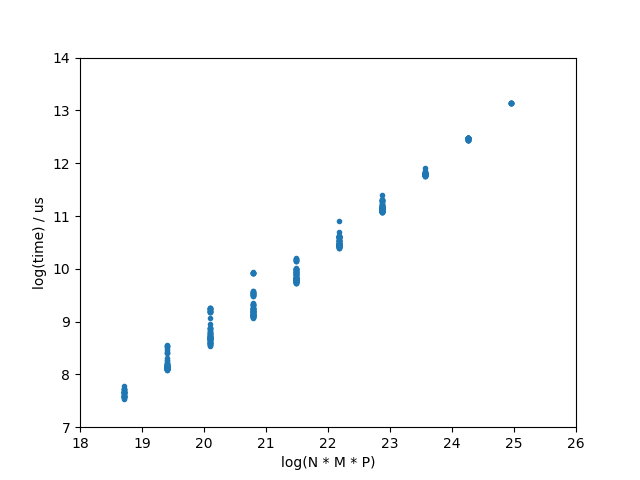
\includegraphics[width=0.8\textwidth]{figures/matmul_cpu_nmp.png}
        \caption{CPU矩阵乘法的性能数据(参数为$N \times M \times P $)}
        \label{fig:matmul_cpu_nmp}
    \end{figure}
    
    \begin{figure}[!htbp]
        \centering
        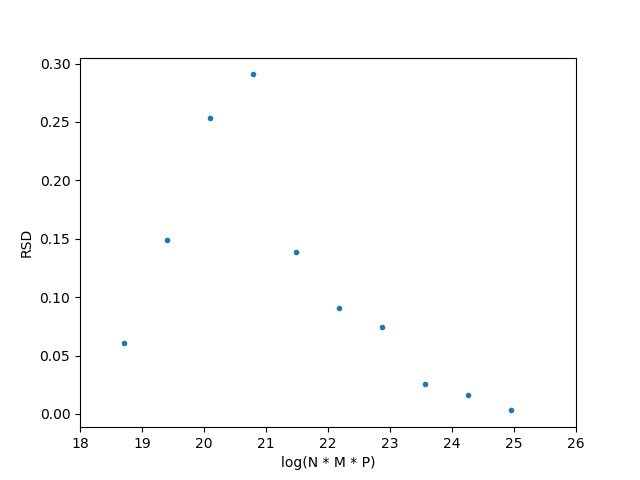
\includegraphics[width=0.8\textwidth]{figures/matmul_cpu_nmp_rsd.png}
        \caption{CPU矩阵乘法的相对标准偏差数据(参数为$ N \times M \times P $)}
        \label{fig:matmul_cpu_nmp_rsd}
    \end{figure}
    
    我们考虑矩阵乘法的并行运行过程,矩阵乘法被拆分成了$ N \times M $个向量点积,每个向量长度为$ P $。因此,我们把$ N \times M $和$ P $作为参数,这时我们发现数据相对$ N \times M $和$ P $都保持了比较好的正比例关系,同时,在固定取值的情况下,相对标准偏差低于0.1,表现在实际数据中,最长的时间相比最短的时间不超过50\%,可以满足我们的预测需求。因此,在CPU上最终的矩阵乘法性能模型采用$ N \times M $和$ P $作为参数,对性能数据进行线性插值,作为预测性能模型。
    
    \begin{figure}[!htbp]
        \centering
        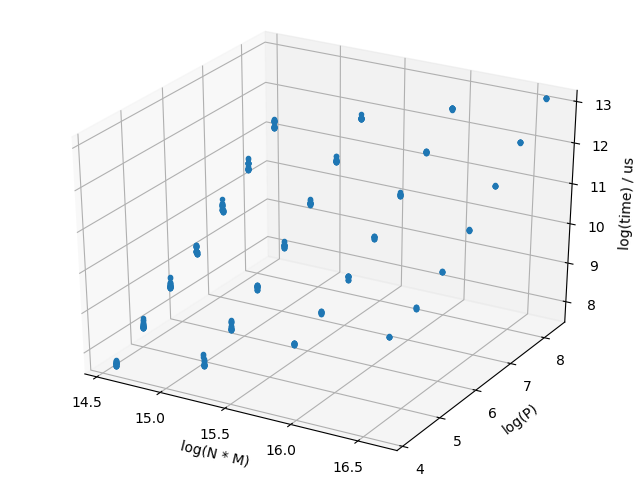
\includegraphics[width=0.8\textwidth]{figures/matmul_cpu_nm_p.png}
        \caption{CPU矩阵乘法的性能数据(参数为$N \times M $和$ P $)}
        \label{fig:matmul_cpu_nm_p}
    \end{figure}

    \begin{figure}[!htbp]
        \centering
        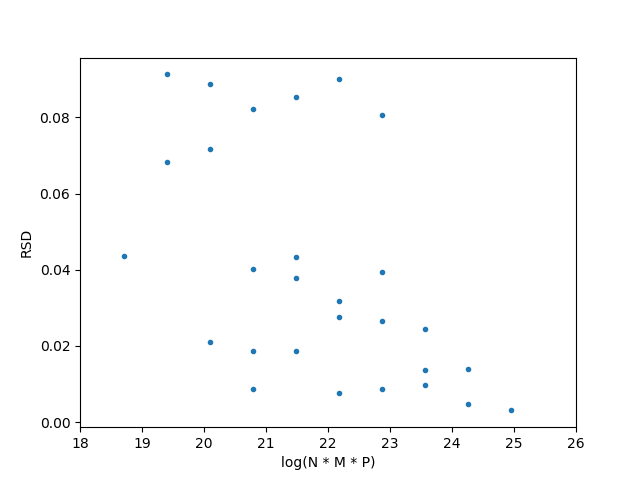
\includegraphics[width=0.8\textwidth]{figures/matmul_cpu_nm_p_rsd.png}
        \caption{CPU矩阵乘法的相对标准偏差数据(参数为$ N \times M $和$ P $)}
        \label{fig:matmul_cpu_nm_p_rsd}
    \end{figure}

    下面我们来对GPU数据进行建模。首先我们观察以$ N \times M \times P $为参数的数据,如图\ref{fig:matmul_gpu_nmp}所示。我们可以观察到,在$ N \times M \times P $取值较大的时候,性能变化较少,而且很符合正比例函数。但是在取值较小的时候关系不明显,而且变化较大。
    
    我们考虑GPU计算矩阵乘法的过程,$ M \times N $代表线程数量,而GPU中线程数量和CPU相比大很多,以我们的实验平台V100为例,V100单卡支持线程数为5120,因此,在$ N \times M \times P $规模不同的时候,性能模型是不同的。
    
    \begin{figure}[!htbp]
        \centering
        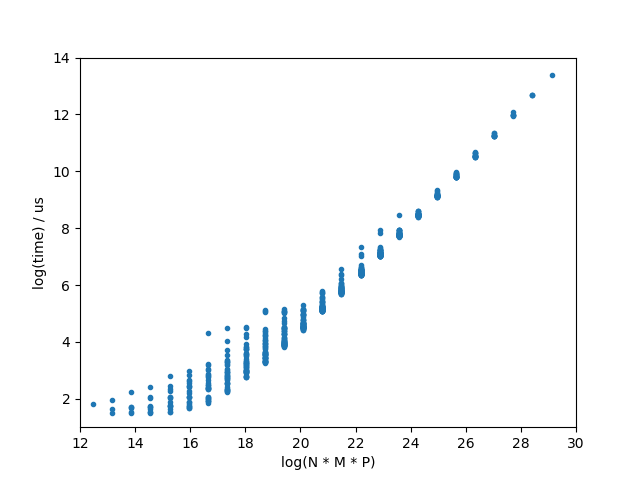
\includegraphics[width=0.8\textwidth]{figures/matmul_gpu_nmp.png}
        \caption{GPU矩阵乘法的性能数据(参数为$N \times M \times P $)}
        \label{fig:matmul_gpu_nmp}
    \end{figure}

    \begin{figure}[!htbp]
        \centering
        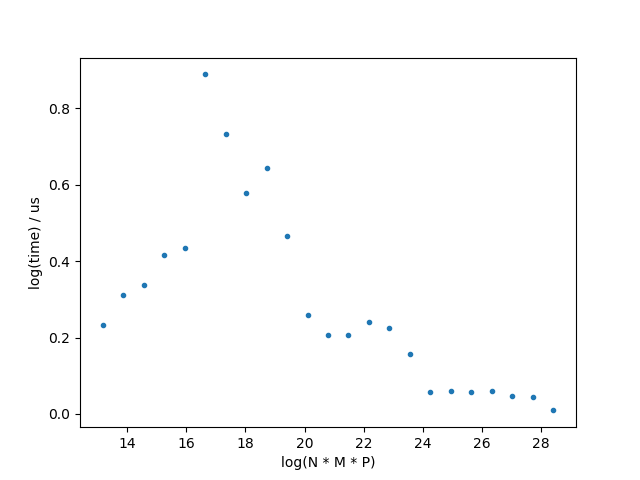
\includegraphics[width=0.8\textwidth]{figures/matmul_gpu_nmp_rsd.png}
        \caption{GPU矩阵乘法的相对标准偏差数据(参数为$ N \times M \times P $)}
        \label{fig:matmul_gpu_nmp_rsd}
    \end{figure}
    
    因为在卷积神经网络中,一般全连接层规模较大,因此我们先考虑大规模的情况。我们把$ N $、$ M $、$ P $规模限制到128以上,性能数据如图\ref{fig:matmul_gpu_nmp_big}所示,我们可以看出,无论是数据的线性程度还是数据的变化范围都有了很大的提升。图\ref{fig:matmul_gpu_nmp_rsd_big}指出,从相对标准偏差值来看,相较图\ref{fig:matmul_gpu_nmp_rsd},GPU在参数取值较大的时候,进使用$ N \times M \times P $为参数,就可以达到比较好的预测效果了。因此,我们在规模较大的时候,直接使用$ M \times N \times P $为参数,进行线性插值。
    
    在规模较小的时候,由于取值数量少,规模小,我们的测试可以较为密集,此时使用$ N $、$ M $、$ P $三个参数进行线性插值,也能得到比较好的预测效果。

    \begin{figure}[!htbp]
        \centering
        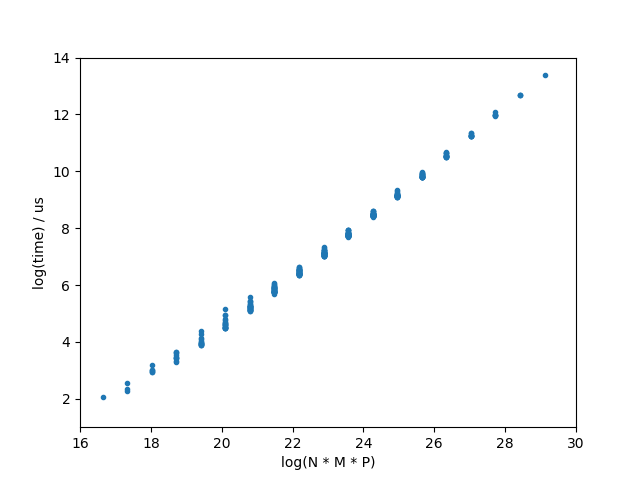
\includegraphics[width=0.8\textwidth]{figures/matmul_gpu_nmp_big.png}
        \caption{GPU矩阵乘法的性能数据(参数为$N \times M \times P $,各参数取值128以上)}
        \label{fig:matmul_gpu_nmp_big}
    \end{figure}

    \begin{figure}[!htbp]
        \centering
        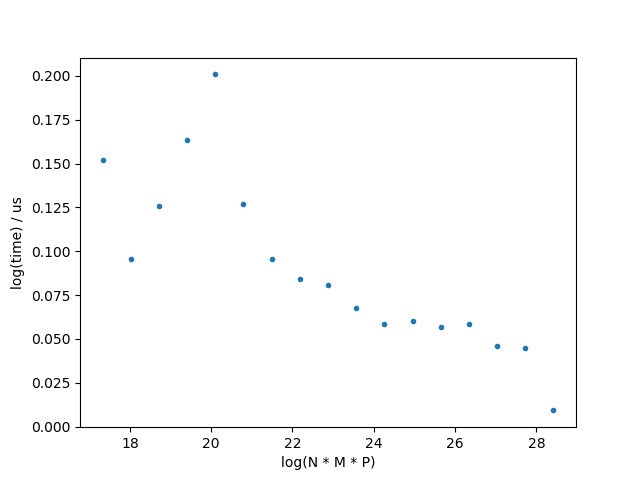
\includegraphics[width=0.8\textwidth]{figures/matmul_gpu_nmp_rsd_big.png}
        \caption{GPU矩阵乘法的相对标准偏差数据(参数为$ N \times M \times P $,各参数取值128以上)}
        \label{fig:matmul_gpu_nmp_rsd_big}
    \end{figure}

\subsection{二维卷积}